\section{CTCLException  Class Reference}
\label{classCTCLException}\index{CTCLException@{CTCLException}}
{\tt \#include $<$TCLException.h$>$}

Inheritance diagram for CTCLException::\begin{figure}[H]
\begin{center}
\leavevmode
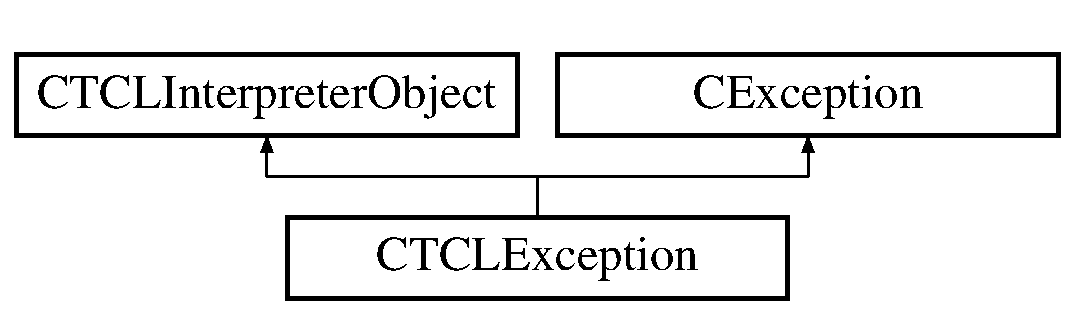
\includegraphics[height=2cm]{classCTCLException}
\end{center}
\end{figure}
\subsection*{Public Methods}
\begin{CompactItemize}
\item 
{\bf CTCLException} ({\bf CTCLInterpreter} \&am\_\-r\-Interpreter, {\bf Int\_\-t} am\_\-n\-Reason, const char $\ast$p\-String)
\item 
{\bf CTCLException} ({\bf CTCLInterpreter} \&am\_\-r\-Interpreter, {\bf Int\_\-t} am\_\-n\-Reason, const std::string \&r\-String)
\item 
virtual {\bf $\sim$CTCLException} ()
\item 
{\bf CTCLException} (const CTCLException \&a\-CTCLException)
\item 
CTCLException {\bf operator=} (const CTCLException \&a\-CTCLException)
\item 
int {\bf operator==} (const CTCLException \&a\-CTCLException)
\item 
{\bf Int\_\-t} {\bf get\-Reason} () const
\item 
void {\bf Add\-Error\-Info} (const char $\ast$p\-Message)
\item 
void {\bf Add\-Error\-Info} (const string \&r\-Message)
\item 
void {\bf Add\-Error\-Info} (const {\bf CTCLString} \&r\-Message)
\item 
void {\bf Set\-Error\-Code} (const char $\ast$p\-Message, const char $\ast$p\-Mnemonic=\char`\"{}???\char`\"{}, const char $\ast$p\-Facility=\char`\"{}TCL\char`\"{}, const char $\ast$p\-Severity=\char`\"{}FATAL\char`\"{})
\item 
void {\bf Set\-Error\-Code} (const string r\-Message, const string \&r\-Mnemonic=string(\char`\"{}???\char`\"{}), const string \&r\-Facility=string(\char`\"{}TCL\char`\"{}), const string \&r\-Severity=string(\char`\"{}FATAL\char`\"{}))
\item 
{\bf CTCLResult} {\bf Get\-Result} () const
\item 
virtual const char $\ast$ {\bf Reason\-Text} () const
\item 
virtual {\bf Int\_\-t} {\bf Reason\-Code} () const
\end{CompactItemize}
\subsection*{Protected Methods}
\begin{CompactItemize}
\item 
void {\bf set\-Interpreter} ({\bf CTCLInterpreter} \&am\_\-r\-Interpreter)
\item 
void {\bf set\-Reason} ({\bf Int\_\-t} am\_\-n\-Reason)
\end{CompactItemize}
\subsection*{Private Attributes}
\begin{CompactItemize}
\item 
{\bf Int\_\-t} {\bf m\_\-n\-Reason}
\end{CompactItemize}


\subsection{Constructor \& Destructor Documentation}
\index{CTCLException@{CTCLException}!CTCLException@{CTCLException}}
\index{CTCLException@{CTCLException}!CTCLException@{CTCLException}}
\subsubsection{\setlength{\rightskip}{0pt plus 5cm}CTCLException::CTCLException ({\bf CTCLInterpreter} \& {\em am\_\-r\-Interpreter}, {\bf Int\_\-t} {\em am\_\-n\-Reason}, const char $\ast$ {\em p\-String})\hspace{0.3cm}{\tt  [inline]}}\label{classCTCLException_a0}




Definition at line 331 of file TCLException.h.

References Int\_\-t, and m\_\-n\-Reason.\index{CTCLException@{CTCLException}!CTCLException@{CTCLException}}
\index{CTCLException@{CTCLException}!CTCLException@{CTCLException}}
\subsubsection{\setlength{\rightskip}{0pt plus 5cm}CTCLException::CTCLException ({\bf CTCLInterpreter} \& {\em am\_\-r\-Interpreter}, {\bf Int\_\-t} {\em am\_\-n\-Reason}, const std::string \& {\em r\-String})\hspace{0.3cm}{\tt  [inline]}}\label{classCTCLException_a1}




Definition at line 339 of file TCLException.h.

References Int\_\-t, and m\_\-n\-Reason.\index{CTCLException@{CTCLException}!~CTCLException@{$\sim$CTCLException}}
\index{~CTCLException@{$\sim$CTCLException}!CTCLException@{CTCLException}}
\subsubsection{\setlength{\rightskip}{0pt plus 5cm}virtual CTCLException::$\sim$CTCLException ()\hspace{0.3cm}{\tt  [inline, virtual]}}\label{classCTCLException_a2}




Definition at line 347 of file TCLException.h.\index{CTCLException@{CTCLException}!CTCLException@{CTCLException}}
\index{CTCLException@{CTCLException}!CTCLException@{CTCLException}}
\subsubsection{\setlength{\rightskip}{0pt plus 5cm}CTCLException::CTCLException (const CTCLException \& {\em a\-CTCLException})\hspace{0.3cm}{\tt  [inline]}}\label{classCTCLException_a3}




Definition at line 351 of file TCLException.h.

References m\_\-n\-Reason.

\subsection{Member Function Documentation}
\index{CTCLException@{CTCLException}!AddErrorInfo@{AddErrorInfo}}
\index{AddErrorInfo@{AddErrorInfo}!CTCLException@{CTCLException}}
\subsubsection{\setlength{\rightskip}{0pt plus 5cm}void CTCLException::Add\-Error\-Info (const {\bf CTCLString} \& {\em r\-Message})\hspace{0.3cm}{\tt  [inline]}}\label{classCTCLException_a9}




Definition at line 410 of file TCLException.h.

References Add\-Error\-Info().\index{CTCLException@{CTCLException}!AddErrorInfo@{AddErrorInfo}}
\index{AddErrorInfo@{AddErrorInfo}!CTCLException@{CTCLException}}
\subsubsection{\setlength{\rightskip}{0pt plus 5cm}void CTCLException::Add\-Error\-Info (const string \& {\em r\-Message})\hspace{0.3cm}{\tt  [inline]}}\label{classCTCLException_a8}




Definition at line 407 of file TCLException.h.

References Add\-Error\-Info().\index{CTCLException@{CTCLException}!AddErrorInfo@{AddErrorInfo}}
\index{AddErrorInfo@{AddErrorInfo}!CTCLException@{CTCLException}}
\subsubsection{\setlength{\rightskip}{0pt plus 5cm}void CTCLException::Add\-Error\-Info (const char $\ast$ {\em p\-Message})}\label{classCTCLException_a7}




Definition at line 313 of file TCLException.cpp.

References CTCLInterpreter::get\-Interpreter(), and CTCLInterpreter\-Object::get\-Interpreter().

Referenced by Add\-Error\-Info().\index{CTCLException@{CTCLException}!getReason@{getReason}}
\index{getReason@{getReason}!CTCLException@{CTCLException}}
\subsubsection{\setlength{\rightskip}{0pt plus 5cm}{\bf Int\_\-t} CTCLException::get\-Reason () const\hspace{0.3cm}{\tt  [inline]}}\label{classCTCLException_a6}




Definition at line 385 of file TCLException.h.

References Int\_\-t, and m\_\-n\-Reason.

Referenced by Reason\-Code().\index{CTCLException@{CTCLException}!GetResult@{GetResult}}
\index{GetResult@{GetResult}!CTCLException@{CTCLException}}
\subsubsection{\setlength{\rightskip}{0pt plus 5cm}{\bf CTCLResult} CTCLException::Get\-Result () const}\label{classCTCLException_a12}




Definition at line 407 of file TCLException.cpp.

References CTCLInterpreter\-Object::get\-Interpreter().

Referenced by Reason\-Text().\index{CTCLException@{CTCLException}!operator=@{operator=}}
\index{operator=@{operator=}!CTCLException@{CTCLException}}
\subsubsection{\setlength{\rightskip}{0pt plus 5cm}CTCLException CTCLException::operator= (const CTCLException \& {\em a\-CTCLException})\hspace{0.3cm}{\tt  [inline]}}\label{classCTCLException_a4}




Definition at line 360 of file TCLException.h.

References m\_\-n\-Reason, CException::operator=(), and CTCLInterpreter\-Object::operator=().\index{CTCLException@{CTCLException}!operator==@{operator==}}
\index{operator==@{operator==}!CTCLException@{CTCLException}}
\subsubsection{\setlength{\rightskip}{0pt plus 5cm}int CTCLException::operator== (const CTCLException \& {\em a\-CTCLException})\hspace{0.3cm}{\tt  [inline]}}\label{classCTCLException_a5}




Definition at line 373 of file TCLException.h.

References m\_\-n\-Reason, CException::operator==(), and CTCLInterpreter\-Object::operator==().\index{CTCLException@{CTCLException}!ReasonCode@{ReasonCode}}
\index{ReasonCode@{ReasonCode}!CTCLException@{CTCLException}}
\subsubsection{\setlength{\rightskip}{0pt plus 5cm}{\bf Int\_\-t} CTCLException::Reason\-Code () const\hspace{0.3cm}{\tt  [virtual]}}\label{classCTCLException_a14}


Returns a code which describes the reason for the exception . This is exception type specific and may be used to do detailed exception analysis and recovery. For example in the {\bf CErrno\-Exception} {\rm (p.\,\pageref{classCErrnoException})} class, the errno at the time of instantiation of the object is returned. The default returns -1 

Reimplemented from {\bf CException} {\rm (p.\,\pageref{classCException_a9})}.

Definition at line 390 of file TCLException.cpp.

References get\-Reason().\index{CTCLException@{CTCLException}!ReasonText@{ReasonText}}
\index{ReasonText@{ReasonText}!CTCLException@{CTCLException}}
\subsubsection{\setlength{\rightskip}{0pt plus 5cm}const char $\ast$ CTCLException::Reason\-Text () const\hspace{0.3cm}{\tt  [virtual]}}\label{classCTCLException_a13}


Returns a const pointer to text which describes the reason the exception was thrown. This is exception type specific. The default action returns a pointer to the constant string: \char`\"{}Unspecified Exception\char`\"{} 

Reimplemented from {\bf CException} {\rm (p.\,\pageref{classCException_a8})}.

Definition at line 374 of file TCLException.cpp.

References Get\-Result().\index{CTCLException@{CTCLException}!SetErrorCode@{SetErrorCode}}
\index{SetErrorCode@{SetErrorCode}!CTCLException@{CTCLException}}
\subsubsection{\setlength{\rightskip}{0pt plus 5cm}void CTCLException::Set\-Error\-Code (const string {\em r\-Message}, const string \& {\em r\-Mnemonic} = string(\char`\"{}???\char`\"{}), const string \& {\em r\-Facility} = string(\char`\"{}TCL\char`\"{}), const string \& {\em r\-Severity} = string(\char`\"{}FATAL\char`\"{}))\hspace{0.3cm}{\tt  [inline]}}\label{classCTCLException_a11}




Definition at line 418 of file TCLException.h.

References Set\-Error\-Code().\index{CTCLException@{CTCLException}!SetErrorCode@{SetErrorCode}}
\index{SetErrorCode@{SetErrorCode}!CTCLException@{CTCLException}}
\subsubsection{\setlength{\rightskip}{0pt plus 5cm}void CTCLException::Set\-Error\-Code (const char $\ast$ {\em p\-Message}, const char $\ast$ {\em p\-Mnemonic} = \char`\"{}???\char`\"{}, const char $\ast$ {\em p\-Facility} = \char`\"{}TCL\char`\"{}, const char $\ast$ {\em p\-Severity} = \char`\"{}FATAL\char`\"{})}\label{classCTCLException_a10}




Definition at line 339 of file TCLException.cpp.

References CTCLInterpreter::get\-Interpreter(), and CTCLInterpreter\-Object::get\-Interpreter().

Referenced by Set\-Error\-Code().\index{CTCLException@{CTCLException}!setInterpreter@{setInterpreter}}
\index{setInterpreter@{setInterpreter}!CTCLException@{CTCLException}}
\subsubsection{\setlength{\rightskip}{0pt plus 5cm}void CTCLException::set\-Interpreter ({\bf CTCLInterpreter} \& {\em am\_\-r\-Interpreter})\hspace{0.3cm}{\tt  [inline, protected]}}\label{classCTCLException_b0}




Definition at line 395 of file TCLException.h.

References CTCLInterpreter\-Object::Bind().\index{CTCLException@{CTCLException}!setReason@{setReason}}
\index{setReason@{setReason}!CTCLException@{CTCLException}}
\subsubsection{\setlength{\rightskip}{0pt plus 5cm}void CTCLException::set\-Reason ({\bf Int\_\-t} {\em am\_\-n\-Reason})\hspace{0.3cm}{\tt  [inline, protected]}}\label{classCTCLException_b1}




Definition at line 399 of file TCLException.h.

References Int\_\-t, and m\_\-n\-Reason.

\subsection{Member Data Documentation}
\index{CTCLException@{CTCLException}!m_nReason@{m\_\-nReason}}
\index{m_nReason@{m\_\-nReason}!CTCLException@{CTCLException}}
\subsubsection{\setlength{\rightskip}{0pt plus 5cm}{\bf Int\_\-t} CTCLException::m\_\-n\-Reason\hspace{0.3cm}{\tt  [private]}}\label{classCTCLException_o0}




Definition at line 321 of file TCLException.h.

Referenced by CTCLException(), get\-Reason(), operator=(), operator==(), and set\-Reason().

The documentation for this class was generated from the following files:\begin{CompactItemize}
\item 
{\bf TCLException.h}\item 
{\bf TCLException.cpp}\end{CompactItemize}
